%-----------------------------------------------------------------------------------
%	PACKAGES AND OTHER DOCUMENT CONFIGURATIONS
%----------------------------------------------------------------------------------



\documentclass[11pt]{article}

\usepackage[top=2cm, bottom=3cm, left=2cm, right=2cm]{geometry}

\setlength{\parindent}{0in}

\newcommand{\Var}{\mathrm{Var}}

\newcommand{\Cov}{\mathrm{Cov}}

\newcommand{\plim}{\rightarrow_{p}}

\usepackage{amsmath, amsfonts}
\usepackage{graphicx}
\usepackage{pdfpages}
\usepackage{bm}
\usepackage{listings}

% Expectation symbol
\newcommand{\E}{\mathrm{E}}
\newcommand{\V}{\mathrm{V}}
\newcommand{\N}{\mathcal{N}}
\newcommand{\R}{\mathbb{R}} 

%----------------------------------------------------------------------------------
%	TITLE AND AUTHOR(S)
%----------------------------------------------------------------------------------

\title{Econ 675 Assignment 1} % The article title


\author{Nathan Mather\thanks{Shouts out to Ani, Paul, Tyler, Erin, Caitlin and others for all the help with this } } % The article author(s) 

\date{\today} % An optional date to appear under the author(s)


%----------------------------------------------------------------------------------
\begin{document}
	
%------------------------------------------------------------------------------
%	TABLE OF CONTENTS & LISTS OF FIGURES AND TABLES
%------------------------------------------------------------------------------
\maketitle % Print the title/author/date block

\setcounter{tocdepth}{2} % Set the depth of the table of contents to show sections and subsections only

\tableofcontents % Print the table of contents


%-------------------------------------------------------------
% Question 1 
%-------------------------------------------------------------
\section{Kernal Density Estimation}
\subsection{Q1 Part 1}

Start by noting that 

$$ \hat{f}^{(s)}(x) = \frac{(-1)^s}{nh^{1+s}} \sum_{i=1}^{n}k^{(s)} \left( \frac{{x}_i - x}{h} \right) 
$$

Now taking the expectation of $\hat{f}^{(s)}(x)$ that we can apply the linearity of expectations to move the expectation inside the sum. Then we can use the i.i.d. assumption to show the sum is just n times the expectation. This leaves us with 

$$  \E[\hat{f}^{(s)}(x)] = \E \left[ \frac{(-1)^s}{h^{1+s}} k^{(s)} \left( \frac{{x}_i - x}{h} \right)  \right]
= \int_{-\infty}^{\infty} \frac{(-1)^s}{h^{1+s}} k^{(s)} \left( \frac{z - x}{h} \right)f(z)dz
$$



Where the second equality is just by the definition of the expectation. Next we use integration by parts. Note that 

$$\int_{-\infty}^{\infty} \frac{(-1)^s}{h^{1+s}} k^{(s)} \left( \frac{z - x}{h} \right)f(z)dz = -\int_{-\infty}^{\infty} \frac{(-1)^s}{h^{s}} k^{(s-1)} \left( \frac{z - x}{h} \right)f^{(1)}(z)dz
$$

Iterating this s times gives us

$$\int_{-\infty}^{\infty} \frac{(-1)^s}{h^{1+s}} k^{(s)} \left( \frac{z - x}{h} \right)f(z)dz
=  (-1)^s \int_{-\infty}^{\infty} \frac{(-1)^s}{h} k \left( \frac{z - x}{h} \right)f^{(s)}(z)dz
= \int_{-\infty}^{\infty} \frac{1}{h} k \left( \frac{z - x}{h} \right)f^{(s)}(z)dz
$$

Next we apply change of variables. let $u = \frac{z - x}{h}$ Note that $du=\frac{1}{h}dz$ so we get 

$$ \int_{-\infty}^{\infty}  k(u)f^{(s)}(x+hu)du $$

Next we Taylor expand $f^{(s)}(x+hu)$ to the $P^{th}$ order about $x$. Recall from properties of the kernal estimator that $ \int_{-\infty}^{\infty}k(u)du = 1$ and that $ \int_{-\infty}^{\infty}k(u)u^jdu = 0$ for all $j\neq p$ This gives us

$$ f^{(s)}(x) +\frac{1}{P!}f^{(s+P)}(x)h^P\int_{-\infty}^{\infty}k(u)u^pdu +o(h^P)
= f^{(s)}(x) +\frac{1}{P!}f^{(s+P)}(x)h^p \mu_P(k) +o(h^P)
$$

which is the desired result. 
\\ \\ 

Now for the variance recall again that 

$$ \hat{f}^{(s)}(x) = \frac{(-1)^s}{nh^{1+s}} \sum_{i=1}^{n}k^{(s)} \left( \frac{{x}_i - x}{h} \right) 
$$

So by the i.i.d. assumption we can get that 

$$ \V \left(\hat{f}^{(s)}(x) \right) = \frac{1}{nh^{2+2s}} \V \left( k^{(s)} \left( \frac{{x}_i - x}{h} \right)  \right)
$$

\begin{align}
\V \left(\hat{f}^{(s)}(x) \right) &= \frac{1}{nh^{2+2s}} \V \left( k^{(s)} \left( \frac{{x}_i - x}{h} \right)  \right)\\
 &= \frac{1}{n2h^{2+2s}} \E \left[\left( k^{(s)} \left( \frac{{x}_i - x}{h} \right)  \right)^2 \right] - \frac{1}{nh^{2+2s}} \E \left[\left( k^{(s)} \left( \frac{{x}_i - x}{h} \right)  \right)^2 \right]^2 \\
  &= \frac{1}{nh^{2+2s}} \E \left[\left( k^{(s)} \left( \frac{{x}_i - x}{h} \right)  \right)^2 \right] - \frac{1}{n}\left( \frac{1}{h^{1+s}} \E \left[\left( k^{(s)} \left( \frac{{x}_i - x}{h} \right)  \right)^2 \right] \right)^2 \\
  &=  \frac{1}{nh^{2+2s}} \int_{-\infty}^{\infty}k^{(s)} \left( \frac{{x}_i - x}{h} \right)^2 f(z)dz +   \frac{1}{nh^{2+2s}} f^{(n)}(X)^2 \\
  &= \frac{1}{nh^{1+2s}} \int_{-\infty}^{\infty} k^{(s)}(u)^2f(x+hu)du + o\left(\frac{1}{nh^{2+2s}} \right)\\
  &= \frac{1}{nh^{1+2s}} \cdot \vartheta_s(K) + o\left(\frac{1}{nh^{2+2s}} \right)
\end{align}

\subsection{Q1 part 2}

We start with the following AMISE
$$ AIMSE[h] = \int \left[ \left( h_n^P \cdot \mu_P(K) \cdot \frac{f^{(P+s)}(x)}{P!}   \right)^2 + \frac{1}{nh_n^{1+2s}} \cdot \vartheta_s(K) \cdot f(x) \right]dx
$$

Using the $\vartheta$ notation so $\vartheta_{P+s}(f) = \int(f^{(P+s)}(x))^2$ and recalling that f(x) integrates to 1 we can rewrite this as 
$$ =  h_n^{2P} \left( \frac{\mu_P(K)}{P!} \right)^2 \vartheta_{P+s}(f) + \frac{\vartheta_s(K)}{nh_n^{1+2s}}
$$
Now taking first order conditions and solving for h 
$$ \frac{d}{dh}AIMSE[h] =  2Ph_n^{2p-1} \left( \frac{\mu_P(K)}{P!} \right)^2 \vartheta_{P+s}(f) -(1+2s) \frac{\vartheta_s(K)}{nh_n^{2+2s}} =0
$$
$$ \implies 2Ph^{1+2P+2s}\left( \frac{\mu_P(K)}{P!} \right)^2 \vartheta_{P+s}(f) = (1+2s) \frac{\vartheta_s(K)}{n}
$$

Thus, we get the AIMSE-optimal bandwidth choice.
$$h_{AIMSE_s} = \left[ \frac{(2s+1)(P!)^2}{2P} \frac{\vartheta_s(K)}{\vartheta_{s+P}(f) \cdot \mu_P(K)^2} \frac{1}{n} \right]^{\frac{1}{1+2P+2s}}$$

Least squares cross-validation is a fully automatic data-driven method of selecting the smoothing parameter h. THis is based on the principle of selecting bandwidth that minimizes the integrated squared error of the resulting estimate.The estimate used is 

$$ \hat{h}_{CV} = \arg \min_{h} \frac{1}{n^2h} \sum_{i=1}^n \sum_{j=1}^n \bar{k} \left(\frac{X_i - X_j}{h}\right) - \frac{2}{n(n-1)h}\sum_{i=1}^n\sum_{j=1, i\neq j}^nk\left(\frac{X_i - X_j}{h}\right)
$$


\subsection{Monte Carlo experiment}

\subsubsection{Q1 Part 3 a} First, we want to compute the theoretically optimal bandwidth for $s=0$, $n=1000$, using the Epanechnikov kernel $(P=2)$, with the following Gaussian DGP:
$$x_i \sim 0.5 \N(-1.5,-1.5) + 0.5\N(1,1)$$

Filling in what we know so far we have : 
$$h_{AIMSE_s} = \left[ \frac{\vartheta_0(K)}{\vartheta_{2}(f) \cdot \mu_2(K)^2} \frac{1}{1000} \right]^{\frac{1}{5}}$$

So we need the second moment of K and the first moment of the second derivative of k squared. We can get two of these values from the table in Bruce Hanson's nonparametric notes. Giving us. 
$$h_{AIMSE_s} = \left[ \frac{\frac{3}{5}}{\vartheta_{2}(f) \cdot \frac{1}{5}^2} \frac{1}{1000} \right]^{\frac{1}{5}}$$

The second derivative of the normal density $\varphi$ with mean $\mu$ variance $\sigma^2$ is 

$$\varphi''_{\mu, \sigma^2}(x) = \frac{1}{\sqrt{2 \pi \sigma^2 }}e^{\frac{-(x-\mu)^2}{2\sigma^2}} \left[ \left( \frac{(x - \mu)}{\sigma^2} \right)^2 - \frac{1}{\sigma^2} \right]
$$

now useing the linearity of integrals we can find $\vartheta_{2}(f)$
$$ \vartheta_{2}(f) = \int_{-\infty}^{\infty} [0.5 \varphi''_{1,1}(x) + 0.5 \varphi''_{-1.5, 1.5}(x)]^2dx \approx 0.03883397
$$

Where the approximation comes from R 

Finally, pluging this in gives the theoretically optimal bandwidth is: 

$$h* = 0.8267532
$$

\subsubsection{Q1 Part 3 b}

Below Is the table of $\widehat{IMSE}^{lI}$ results and $\widehat{IMSE^{LO}}$ results by bandwidth $h$. My stata code was significantly slower and so I only ran 10 repetitions. Even with that the plots give us generally the same idea. \\ \\ 
R TABLE
\begin{center}
	% latex table generated in R 3.3.2 by xtable 1.8-2 package
% Tue Oct 09 02:55:44 2018
\begin{tabular}{lll}
  \hline
imse\_li & imse\_lo & h \\ 
  \hline
0.000166 & 0.000166 & 0.5 \\ 
  0.000144 & 0.000145 & 0.6 \\ 
  0.000124 & 0.000126 & 0.7 \\ 
  0.000119 & 0.000122 & 0.8 \\ 
  0.000106 & 0.000109 & 0.9 \\ 
  0.000124 & 0.000127 & 1 \\ 
  0.00013 & 0.000133 & 1.1 \\ 
  0.000151 & 0.000154 & 1.2 \\ 
  0.00019 & 0.000194 & 1.3 \\ 
  0.000215 & 0.000218 & 1.4 \\ 
  0.000263 & 0.000267 & 1.5 \\ 
   \hline
\end{tabular}

\end{center}

STATA TABLE
\begin{center}
	

\begin{tabular}{lcc} \hline
h & m\_imse\_li & m\_imse\_lo \\ \hline
0.500 & 0.000110 & 0.000110 \\
0.600 & 8.51e-05 & 8.62e-05 \\
0.700 & 6.99e-05 & 7.16e-05 \\
0.800 & 6.21e-05 & 6.42e-05 \\
0.820 & 6.14e-05 & 6.36e-05 \\
0.900 & 6.17e-05 & 6.42e-05 \\
1 & 6.80e-05 & 7.09e-05 \\
1.100 & 8.06e-05 & 8.38e-05 \\
1.200 & 9.89e-05 & 0.000102 \\
1.300 & 0.000123 & 0.000127 \\
1.400 & 0.000153 & 0.000157 \\
 1.500 & 0.000188 & 0.000192 \\ \hline
\end{tabular}


\end{center}


My graphs from both programs are below 

\begin{center}
		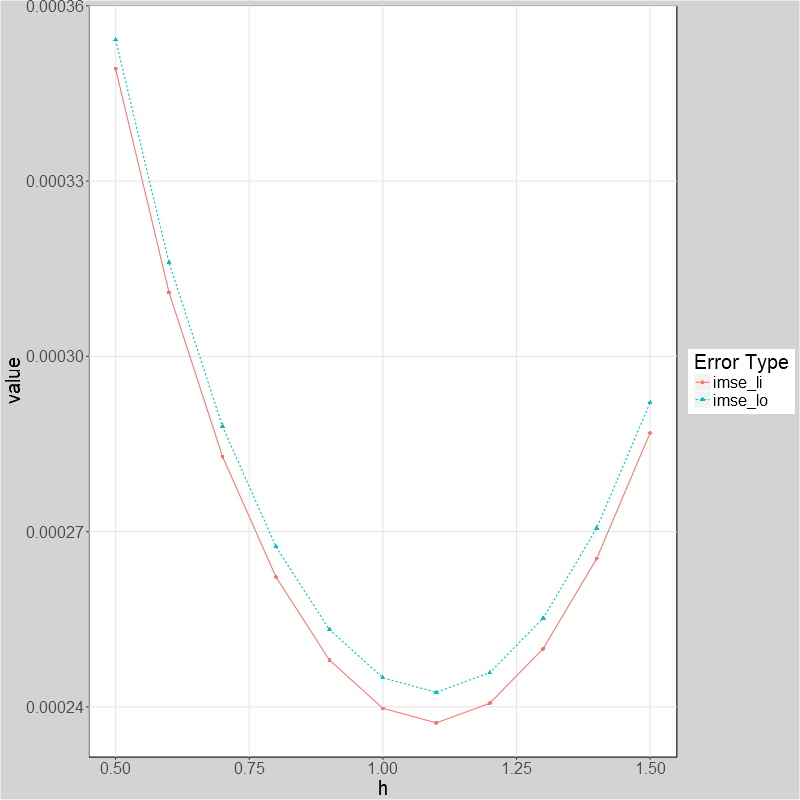
\includegraphics[width=.6\linewidth]{plot_1_3_b.png}

\end{center}
\begin{center}
	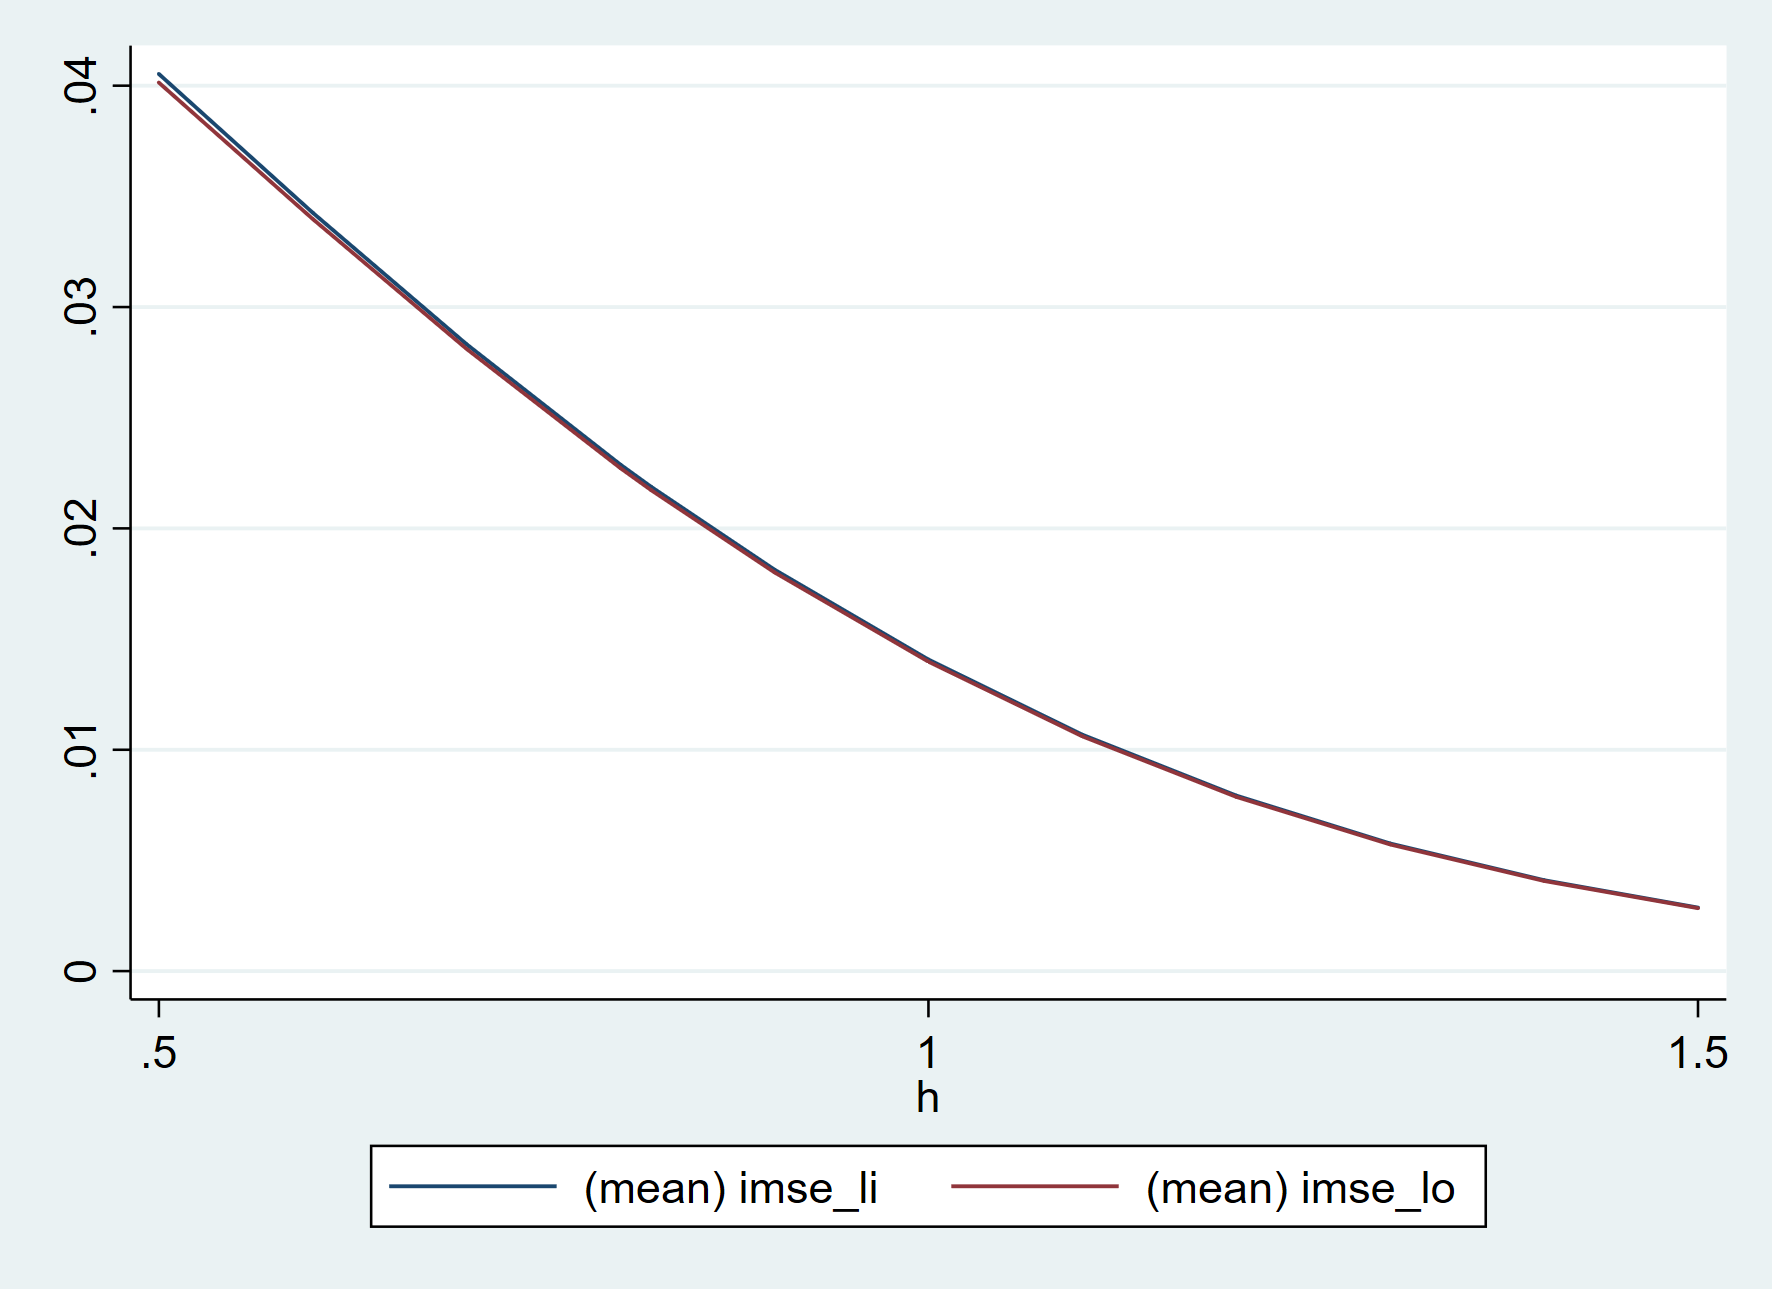
\includegraphics[width=.6\linewidth]{stata_plot_1_3_b.png}
	
\end{center}


\subsubsection{Q1 Part 3 c}
Intuitively the difference between the two estimators, LI and LO, is that the LI includes the extra zero term in the sum since we include $x_i - x_i$. As the size of the sample increases this contribution to the overal average will go to zero. Meaning that the LI IMSE will also converge to the correct estimate. s


\subsubsection{Q1 Part 3 d}
The "d\_h\_hat" column of the graph in part c is my calculation of this over the 1000 iterations. The value it came up with was 1.04. This is somewhat close but, as expected, not exactly correct. 

\section{Question 2: Linear Smoothers, Cross-validation and Series}

\subsection{Q2 Part 1}
For local polynomial regression we want to estimate $e(x) = \E[y_i|x_i = x]$. The idea of a local polynomial regression is to estimate e(x) around the point x using a polynomial of degree p. We estimate this polynomial with weighted least squares. For a given x, we want to solve. 

$$\hat{\bm{\beta}}_{LP}(x) = \arg \min_{\beta \in \R^{p+1}} \sum_{i=1}^{n}[y_i - \bm{r}_p(x_i - x)'\bm{\beta}]^2K(\frac{x_i-x}{h})
$$

where $ \bm{r}_p(x) = (1,x,x^2,...,x^p)'$ and $\hat{e}(x) = \hat{\beta}_0$

from the lecture notes we can get that 
$$\hat{\bm{\beta}}_{LP}(x) = (\bm{R'_pWR'_p})^{-1}\bm{R'_pWy}
$$

I think This simplifies to the following 
$$\hat{e}(x)= e'_1 \left( \sum_{i=1}^{n} \bm{r}_p(x_i-x)\bm{r}_p(x_i-x)'w_i\right)^{-1} \left( \sum_{i=1}^{n} \bm{r}_p(x_i - x)w_iy_i \right)
$$

where $ wi = K(\frac{x_i - x}{h}) $

Now for the series estimation. 
$$  \bm{\hat{\beta}_{series}} = \arg \min_{\beta \in \R^{p+1}} \sum_{i=1}^{n}(y_i -\bm{r}_p(x_i)'\bm{\beta})^2
	$$
	
where $ \bm{r}_p(x_i) = (1,x_x,x_i^2, ..., x_i^p)$ and 

$$\hat{e}(x) = \bm{r}_p(x)'\hat{\bm{B}}_{series}$$

Together we get 
$$ \hat{\bm{B}}_{series} = (\bm{R}`_p \bm{R}_p)^{-1}\bm{R}_p\bm{y}
$$

so 
$$\hat{e}(x) = \bm{r}_p(x)'(\bm{R}`_p \bm{R}_p)^{-1}\bm{R}_p\bm{y}$$

Writing this in linear summation form I believe we get 
$$\hat{e}(x) =  \bm{r}_p(x)' \left( \sum_{i=1}^{n}\bm{r}_p(x_i)\bm{r}_p(x_i)'\right)^{-1} \left( \sum_{i=1}^{n} \bm{r}_p(x_i)y_i \right)$$

\subsection{Q2 Part 2}
We want to choose the tuning parameter to minimize the mean squared leave one out error which is 

$$\hat{c} = \arg \min_{c} \frac{1}{n} \sum_{i=1}^{n}(y_i - \hat{e}_(i)(x_i;c))^2$$

where $\hat{e}_{(i)}(x_i)$ is the estimator of the regression function that leaves out $x_i$

We can write the local polynomial series estimator as 
$$ \hat{\bm{e}}(x) = \bm{Sy}$$

Where S is the smoothing matrix. Note that the rows of S sum to one so $\bm{S1 = 1}$. For the leave one out estimator we want to use $\bm{S}$ but with the $i_{th}$ row and column removed. If we let the elements of $\bm{s}$ be denoted by $w_{ij}$ than deleting the $i_{th}$ column means that the $i_{th}$ row will now sum to $1-w_{ij}$. So, we divide by $1-w_{ij}$ to renormalize and get the the leave-one-out estimator is 
$$\hat{e}_{(i)}(x_i) = \frac{1}{1-w_{ij}} \sum_{j=1 j\ne i}^{n} w_{ij} y_i$$

The full sample estimator is 
$$\hat{e}(x_i) = \sum_{j=1}^{n}w_{ij}y_i$$

Together we can get that 
$$\hat{e}_{(i)}(x_i)(1-w_{ij}) =  \sum_{j=1 j\ne i}^{n} w_{ij} y_i
$$

$$\implies \hat{e}_{(i)}(x_i)=  \sum_{j=1 j\ne i}^{n} w_{ij} y_i + w_{ij}\hat{e}_{(i)}(x_i) = \sum_{j=1}^{n} w_{ij} y_i + w_{ij}\hat{e}_{(i)}(x_i)-w_{ij}y_i = \hat{e}_{(i)}(x_i) + w_{ij}\hat{e}_{(i)}(x_i)-w_{ij}y_i$$

$$ \implies y - \hat{e}_{(i)}(x_i) = y - \hat{e}_{(i)}(x_i) - w_{ij}\hat{e}_{(i)}(x_i)+w_{ij}y_i$$
$$ = y- \hat{e}_{(i)}(x_i) + w_{ij}(y_{i} - \hat{e}_{(i)}))
$$ 

$$\implies y_i - \hat{e}_{(i)}(x_i) = \frac{1}{1-w_{ij}}(y_i - \hat{e}(x_i))
$$

Which is what we wanted 

\subsection{Q2 part 3}
Note that we have iid data and the $\sum_{i=1}^{n}w_{n,i}(x_i)=1$ first we want to find 

$$ \E[\hat{e}(x)|\bm{x}] = \E\left[ \sum_{i=1}^{n} w_{n,i}(x_i)y_i|\bm{x} \right] = \sum_{i=1}^{n}\E\left[  w_{n,i}(x_i)y_i|\bm{x} \right]= \sum_{i=1}^{n}  w_{n,i}(x_i) \E\left[ y_i|\bm{x} \right] = \E[y_i|\bm{x}]
$$

Now as long as we have a bounded second moment we can use CLT to get asymptotic normality. Now to calculate the variance:

$$ \V[\hat{e}(x)|\bm{x}] = \V \left[ \sum_{i=1}^{n} w_{n,i}(x_i)y_i |\bm{x}  \right] =  \sum_{i=1}^{n} \V \left[ w_{n,i}(x_i)y_i |\bm{x}  \right] = \sum_{i=1}^{n} w_{n,i}(x_i)^2 \V \left[y_i |\bm{x}  \right]
$$

Then if we assume homoroskedasticity we get the estimator

$$\hat{\V}(x) = \hat{\sigma}^2 \sum_{i=1}^{n}w_{n,i}(x)^2$$

	
Where 
$\hat{\sigma}^2 = \frac{1}{n-1} \sum_{i=1}^{n} (y_i - \hat{e}(x_i))^2$

\subsection{Q2 part 4}

The pointwise asymptotically valid $95\% $ convidence interval for $e(x)$ is 
$$CI_{95}(x) = [\hat{e}(x) - 1.96 \sqrt{\hat{\V}(x)}, \hat{e}(x) + 1.96 \sqrt{\hat{\V}(x)}] $$

This is just a confidence interval for a given point. applying this to a grid of points across the line and interpreting that as a band for the function is incorrect. For uniformly valid inference we need that the estimate is less that the cutoff for all values of x, not just one specific x. 

\subsection{Q2 part 5}
\subsubsection{Q2 part 5 a}
See the code in appendix 

\subsubsection{Q2 part 5 B} 
The plot of the CV(K) simulations is below 
\begin{center}
	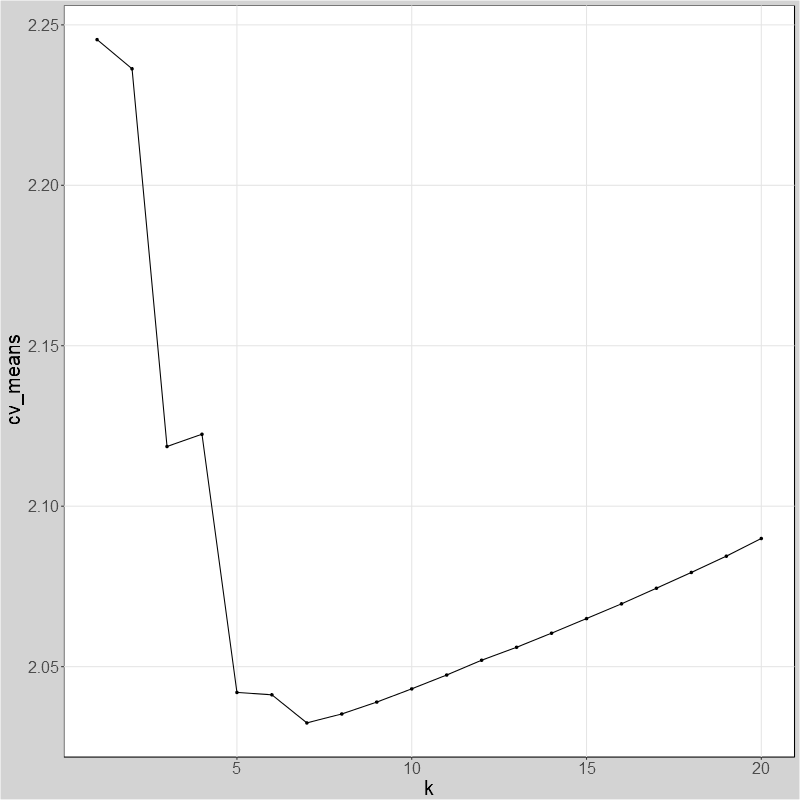
\includegraphics[width=.6\linewidth]{plot_2_5_b.png}
	
\end{center}

\begin{center}
	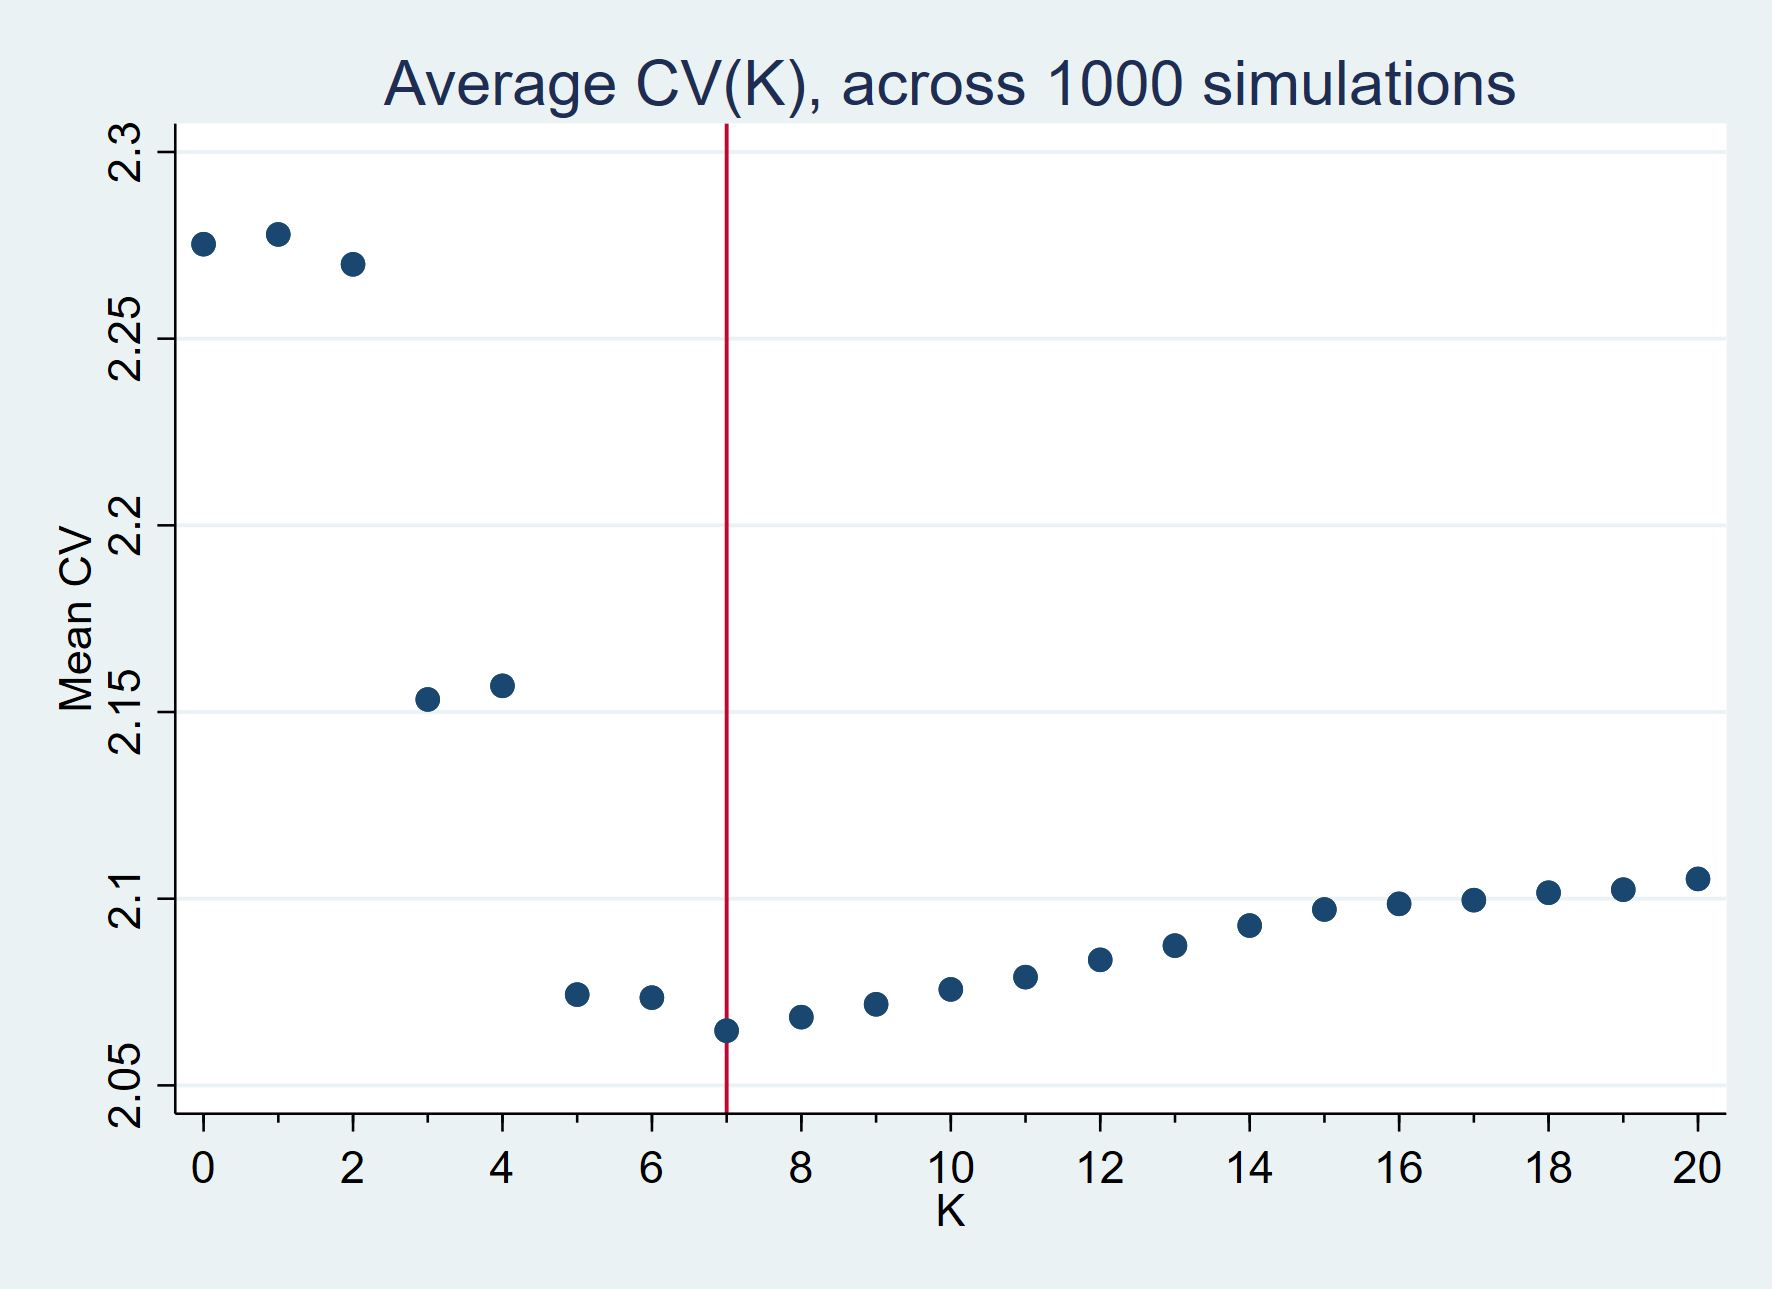
\includegraphics[width=.6\linewidth]{stata_plot_2_5_b.png}
	
\end{center}





\subsection{ Q2 part 5 C}
My plot is below. I used homoscedastic standard errors.  The dotted line is my estimate
\begin{center}
	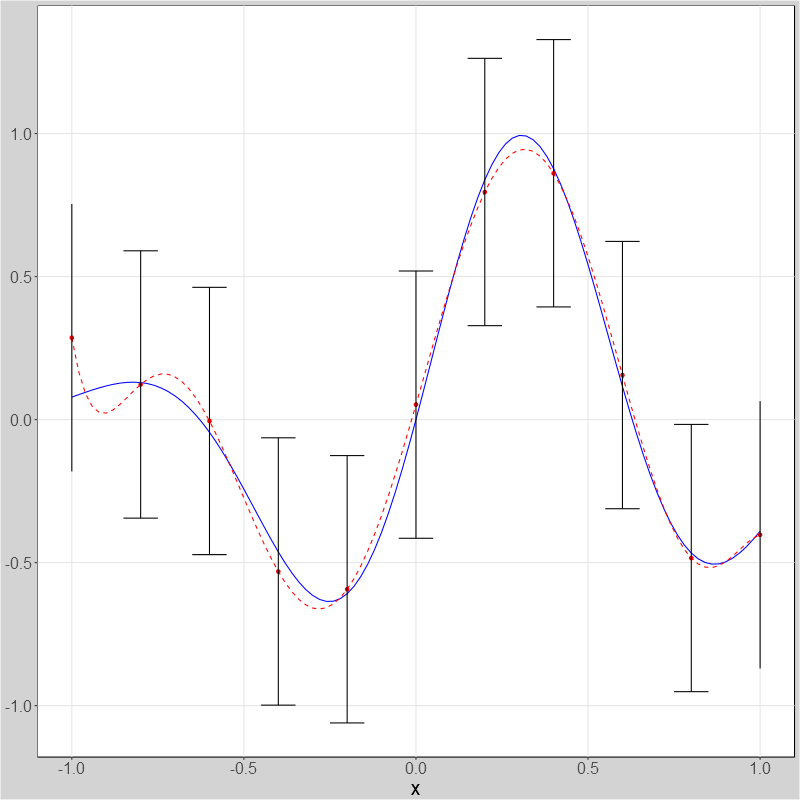
\includegraphics[width=.6\linewidth]{plot_2_5_c.png}
	
\end{center}
\begin{center}
	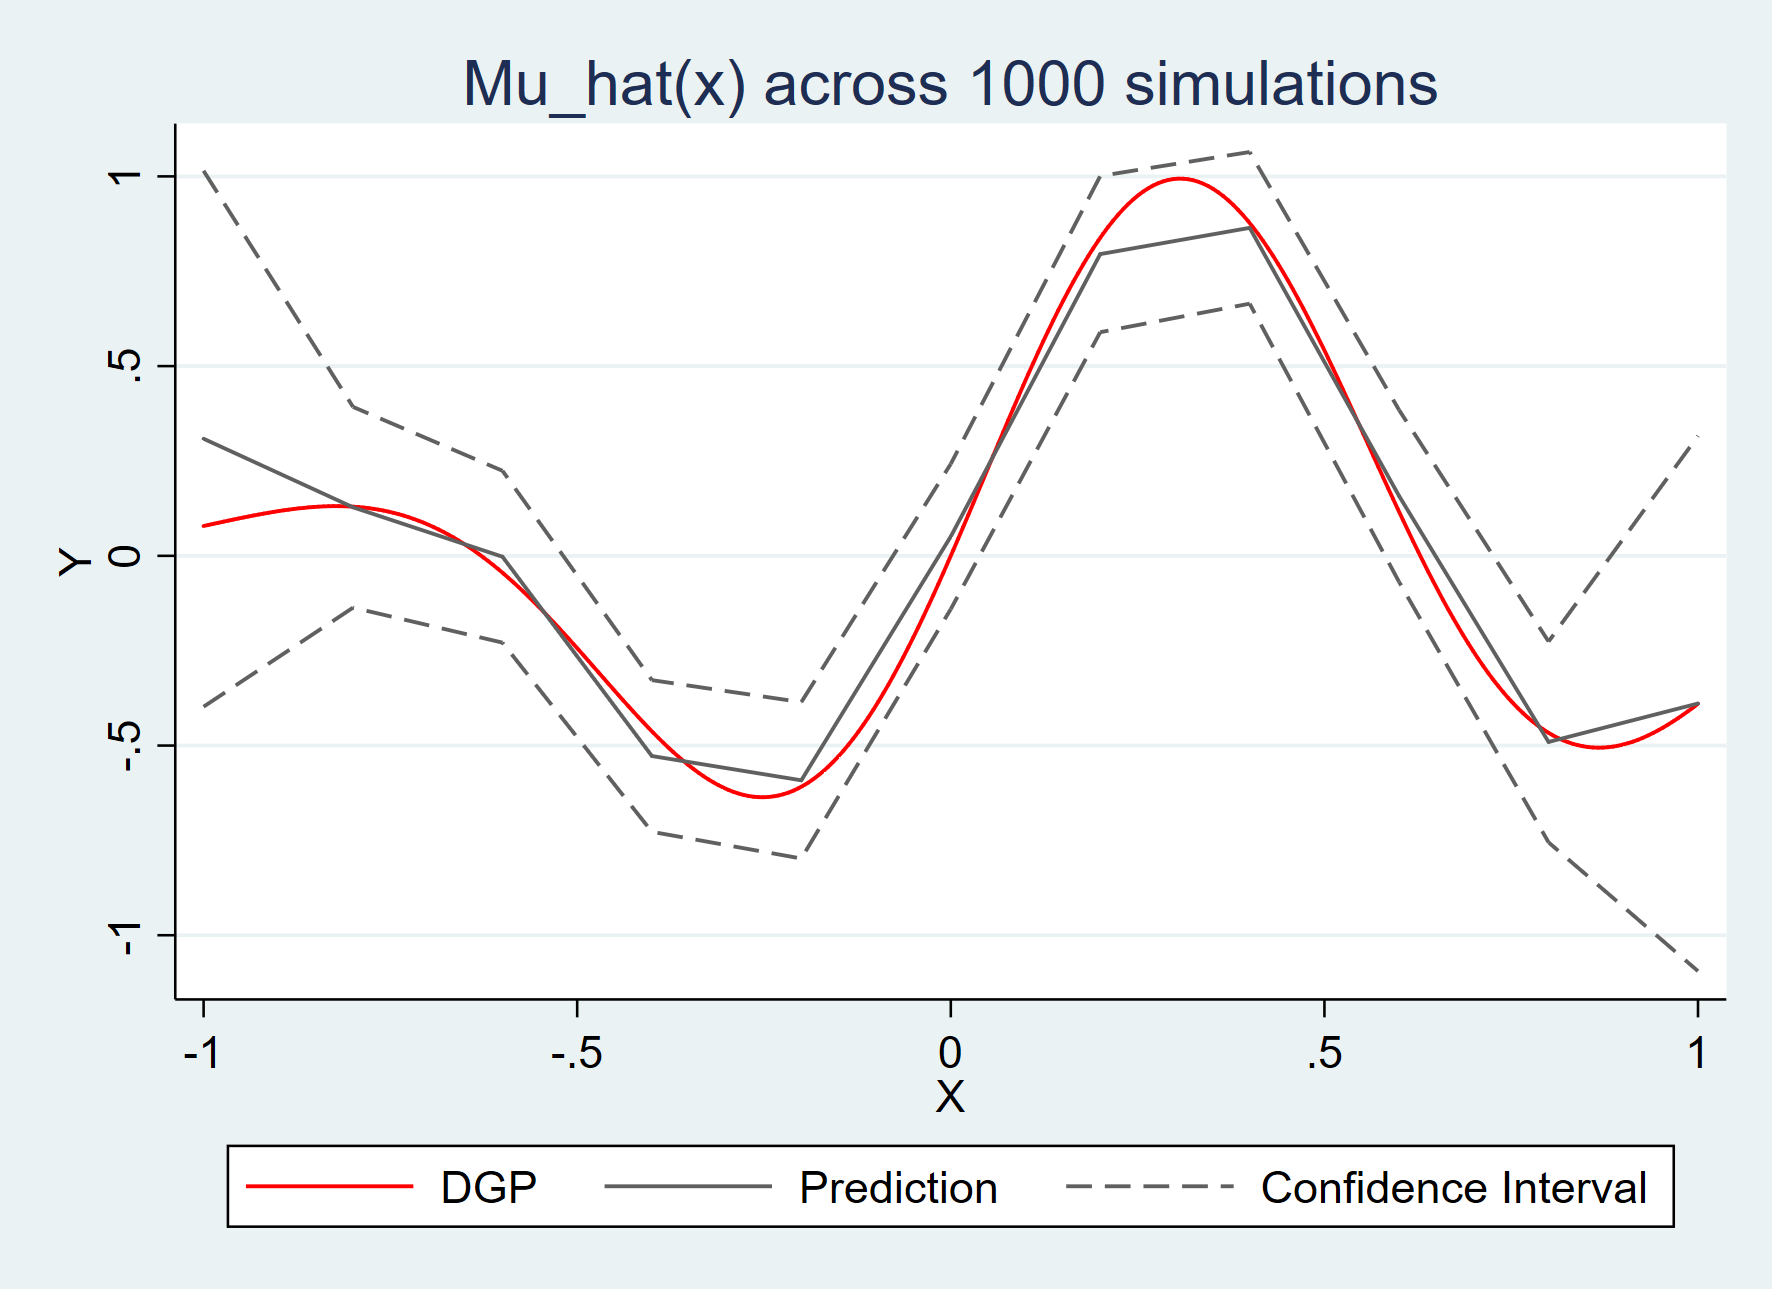
\includegraphics[width=.6\linewidth]{stata_plot_2_5_c.png}
	
\end{center}



\subsection{Q2 part 5 D}
Calculating the derivative of $u(x)$ we get 
$$ e^{(0.1\cdot(4x-1)^2)}[5 \cdot cos(5x) - 0.8 \cdot (4x-1)sin(5x)]
$$

Taking the derivative of the estimated euqation we get 
$$\hat{u}'(x) = \beta_1 + 2\beta_2x + 3\beta_3x^2 + 4\\beta_4x^3 + 5\beta_5x^4 + 6\beta_6x^5 + 7\beta_7x^6$$

I plot the corresponding curves below. The dotted line is my estimate 
\begin{center}
	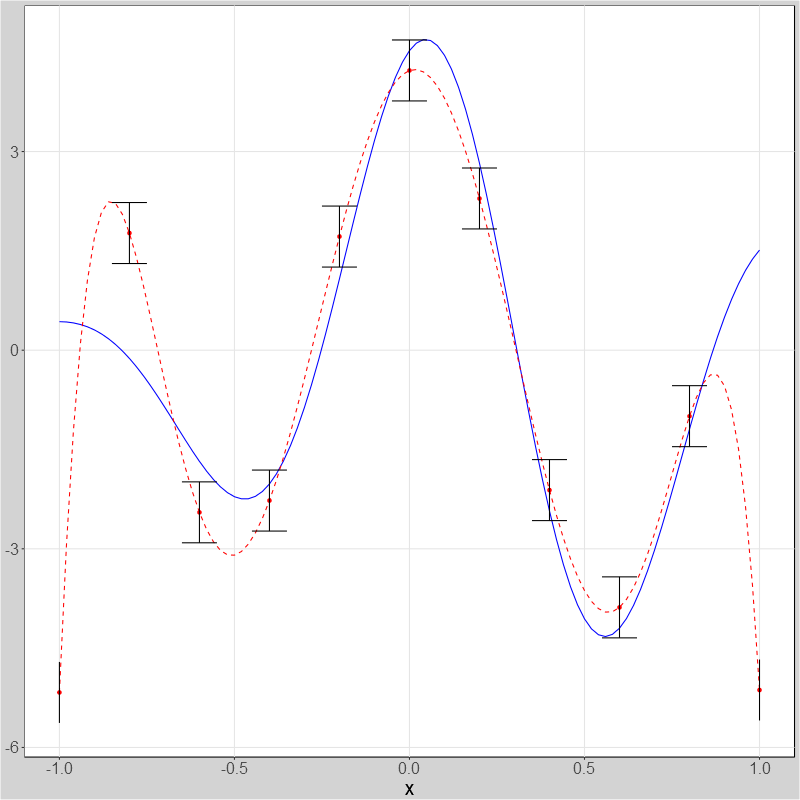
\includegraphics[width=.6\linewidth]{plot_2_5_d.png}
	
\end{center}

\begin{center}
	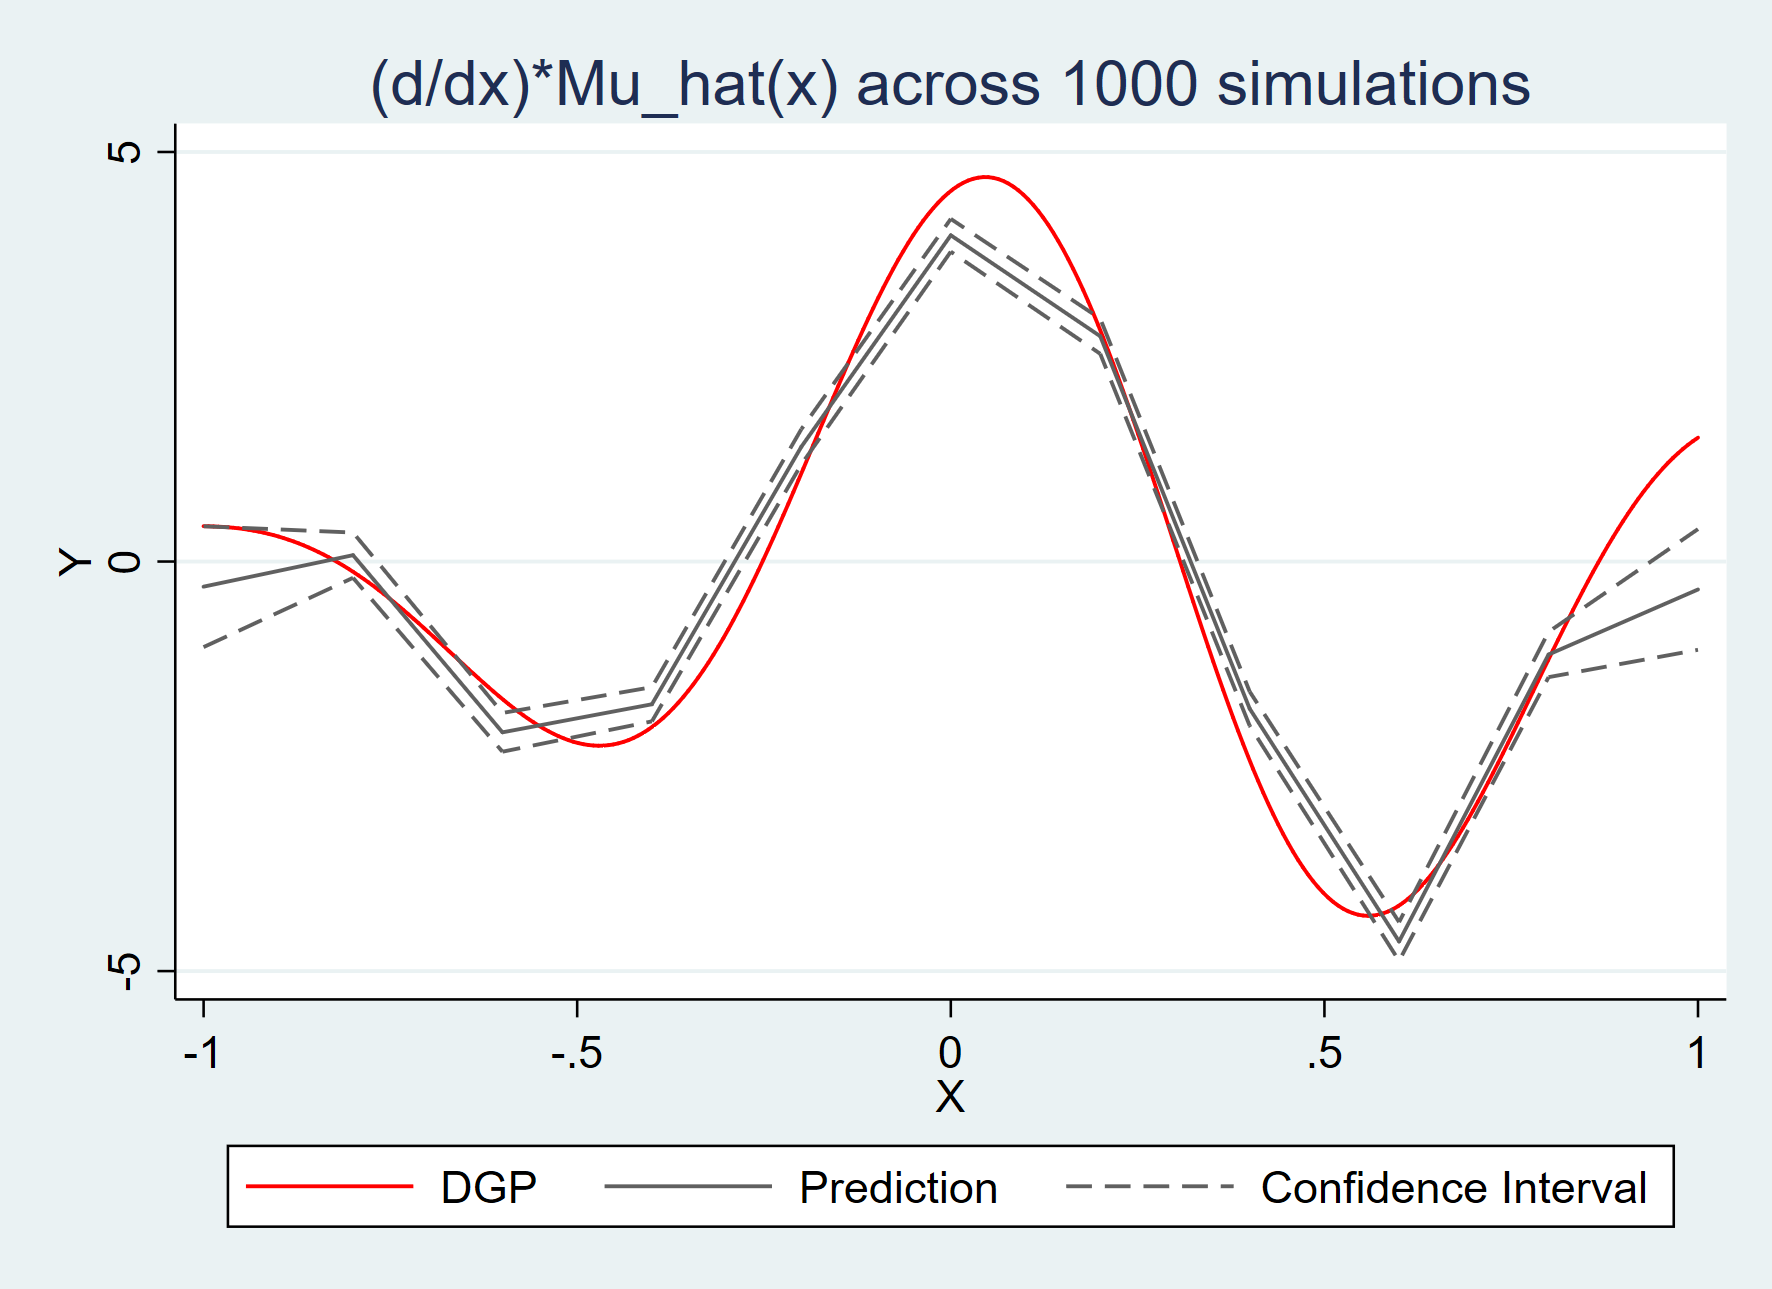
\includegraphics[width=.6\linewidth]{stata_plot_2_5_d.png}
	
\end{center}


\section{Question 3: Semiparametric Semi-Linear Model }
\subsection{Q3 part 1}
first note that $\theta_0$ cannot contain a constant. since $\alpha + g(z) = [\alpha + c] + [g(z) - c] \equiv \alpha_{new} + g_{new}(z)$ the sum of the new g and intercept are observationally equivalent to the old ones so they cannot be identified. From Li and Racine page 223 we can see that the requirements for identifiability are that  $\E[(t_i - h_0(x_i))(t_i - h_0(x_i))']$ is positive definite. 3
\\
\\
To prove the moment condition let's start with the expectation of interest and apply the law of iterated expectations. 

$$ \E[(t_i - h_o(x_i))(y_i - t_i \theta_0)] = \E[\E[(t_i - h_o(x_i))(y_i - t_i \theta_0) |x_i]] = \E[\E[(t_i - h_o(x_i))(g_0(x_i) + \epsilon_i) |x_i]]
$$

$$ = \E[\E[(t_i - h_o(x_i))g_o(x_i)|x_i]] + \E[\E[(t_i - h_o(x_i))\epsilon_i|x_i]] 
$$
$$ = \E[g_o(x_i)\E[(t_i - h_o(x_i))|x_i]] + \E[(t_i - h_o(x_i))\E[\epsilon_i|x_i, i_i]] = 0 $$

Now to find a closed form solution for $\theta_0$. 

$$ \E[(t_i - h_o(x_i)y_i )] - \E[(t_i - h_o(x_i)t_i)] \theta_0 = 0$$
$$ \implies \theta_0= \frac{\E[(t_i - h_o(x_i)y_i )] }{\E[(t_i - h_o(x_i)t_i)]}
$$

The IV interpretation can be given as follows. Let $yi=t_i \theta_0 + g_0(x_i) + \epsilon_i = t_i \theta_0 + \mu_i$. Now $\mu_i$ is uncorrelated with $t_i$ so we can define and instrument $z_i = t_i - h_0(x_i) $ which has the property of $\E[z_i\mu_i] = 0$ and $\E[t_iz_i] \neq 0$ so it is a valid instrument. 

\subsection{Q3 part 2}
\textbf{(a)} As the question asks we will consider the power series approximation. 
$$\E[y_i|\bm{x}_i] \approx t_i \theta_0 + \bm{p}^K(\bm{x}_i)'\bm{\gamma}_k
$$

Next, as the question instructs, we can use the partition regression formula and get the OLS estimator 
$$\hat{\theta}(K) = (\bm{t'M_xt})^{-1}\bm{t'M_xY}
$$

Where here $\bm{t} = (t_1,..., t_n)'$ and 
$\bm{M}_p = \bm{I - P_{r_p(x)}}$ \\ \\
and $ \bm{P_{r_p(x)}} = \bm{R_p(R'_pR_p)^{(-1)}R'_p} $

$$
\bm{R}_p = 
\begin{bmatrix}
	1 & (\bm{x}_1) & (\bm{x}_1)^2 & \dots& (\bm{x}_1)^p \\
	1 & (\bm{x}_2) & (\bm{x}_2)^2 & \dots& (\bm{x}_2)^p\\
	\vdots & \vdots & \vdots & \ddots & \vdots \\
	1 & (\bm{x}_n) & (\bm{x}_n)^2 & \dots& (\bm{x}_n)^p
\end{bmatrix}
$$

\textbf{(b)}

We used the moment condition when discussing the IV estimate interpretation in part 1 to find
$$\theta_0= \frac{\E[(t_i - h_o(x_i)y_i )] }{\E[(t_i - h_o(x_i)t_i)]}$$

So we can estimate this with 
$$\left(\frac{1}{n} \sum_{i=1}^{n}t_i - h_o(x_i)t_i \right)^{-1}\left(\frac{1}{n} \sum_{i=1}^{n}t_i - h_o(x_i)y_i \right) $$

\subsection{Q3 part 3}
\textbf{(a)}

WE can just use the partialing out method above to get 
$$\hat{\theta}(K) = (\bm{t'M_pt})^{-1}\bm{t'M_p}(\bm{t} \theta_0 + \bm{R_p \gamma_k} + \bm{e}) = \theta + (\bm{t'M_pt})^{-1} \bm{t'M_pe}$$
Now with iid data and conditional l heteroskedasticity, we can use the WLLN and CLT as usual to get normality and the sandwich form variance matrix 

\textbf{(b)}

The asymptotically valid 95\% confidence interval is just the same as usual then

$$ CI_{95} = [\hat{\theta}(K) - 1.96\sqrt{V_{HCO}},\hat{\theta}(K) + 1.96\sqrt{V_{HCO}} ]
$$ 

\subsection{Q3 part 4}
\subsubsection{Q3 part 4 a}
see code in appendix 
\subsubsection{Q3 part 4 b}

My results from R are in the table below 

\begin{center}
	% latex table generated in R 3.3.2 by xtable 1.8-2 package
% Thu Oct 11 23:41:17 2018
\begin{tabular}{rrrrrr}
  \hline
K & Theta & Bias & S.D & V\_HCO & Rejection rate \\ 
  \hline
6.000 & 1.988 & 0.428 & 4.135 & 0.551 & 1.000 \\ 
  11.000 & -0.388 & 0.249 & 0.212 & 0.280 & 0.300 \\ 
  21.000 & -0.403 & 0.263 & 0.232 & 0.284 & 0.300 \\ 
  26.000 & -0.387 & 0.262 & 0.219 & 0.284 & 0.300 \\ 
  56.000 & -0.319 & 0.304 & 0.194 & 0.278 & 0.200 \\ 
  61.000 & -0.320 & 0.314 & 0.201 & 0.265 & 0.300 \\ 
  126.000 & -0.016 & 0.090 & 0.008 & 0.139 & 0.000 \\ 
  131.000 & -0.021 & 0.085 & 0.008 & 0.138 & 0.000 \\ 
  252.000 & -0.080 & 0.146 & 0.028 & 0.128 & 0.200 \\ 
  257.000 & -0.076 & 0.139 & 0.025 & 0.128 & 0.200 \\ 
  262.000 & -0.085 & 0.134 & 0.025 & 0.128 & 0.200 \\ 
  267.000 & -0.101 & 0.142 & 0.030 & 0.129 & 0.200 \\ 
  272.000 & -0.112 & 0.133 & 0.030 & 0.129 & 0.200 \\ 
  277.000 & -0.115 & 0.137 & 0.032 & 0.130 & 0.200 \\ 
   \hline
\end{tabular}

\end{center}

\begin{center}
	
\begin{tabular}{lccccc} \hline
theta\_hat & se\_hat & bias & cov & svar & K \\ \hline
3.002 & 0.114 & 2.002 & 0 & 0.688 & 1 \\
0.734 & 0.140 & -0.266 & 0.00500 & 0.249 & 2 \\
0.734 & 0.140 & -0.266 & 0.00500 & 0.249 & 3 \\
0.766 & 0.139 & -0.234 & 0.00600 & 0.223 & 4 \\
0.766 & 0.139 & -0.234 & 0.00600 & 0.223 & 5 \\
0.796 & 0.139 & -0.204 & 0.00500 & 0.256 & 6 \\
0.796 & 0.139 & -0.204 & 0.00500 & 0.256 & 7 \\
0.790 & 0.139 & -0.210 & 0.00600 & 0.259 & 8 \\
0.790 & 0.139 & -0.210 & 0.00600 & 0.259 & 9 \\
0.793 & 0.139 & -0.207 & 0.00500 & 0.250 & 10 \\
0.791 & 0.139 & -0.209 & 0.00600 & 0.230 & 11 \\
0.779 & 0.139 & -0.221 & 0.00600 & 0.242 & 12 \\
0.771 & 0.139 & -0.229 & 0.00700 & 0.227 & 13 \\
 0.795 & 0.138 & -0.205 & 0.00700 & 0.220 & 14 \\ \hline
\end{tabular}


\end{center}


\subsubsection{Q3 part 4 c}

Using cross-validation, I get $\hat{K}_{cv} = 126$. We can see from Table 1, across the simulations,
$\hat{K}_{cv}$ gives a  low rejection rate, but other estimators have lower bias and variance.

\section{Appendix}
\subsection{R Code}
Here is the graph from R 
 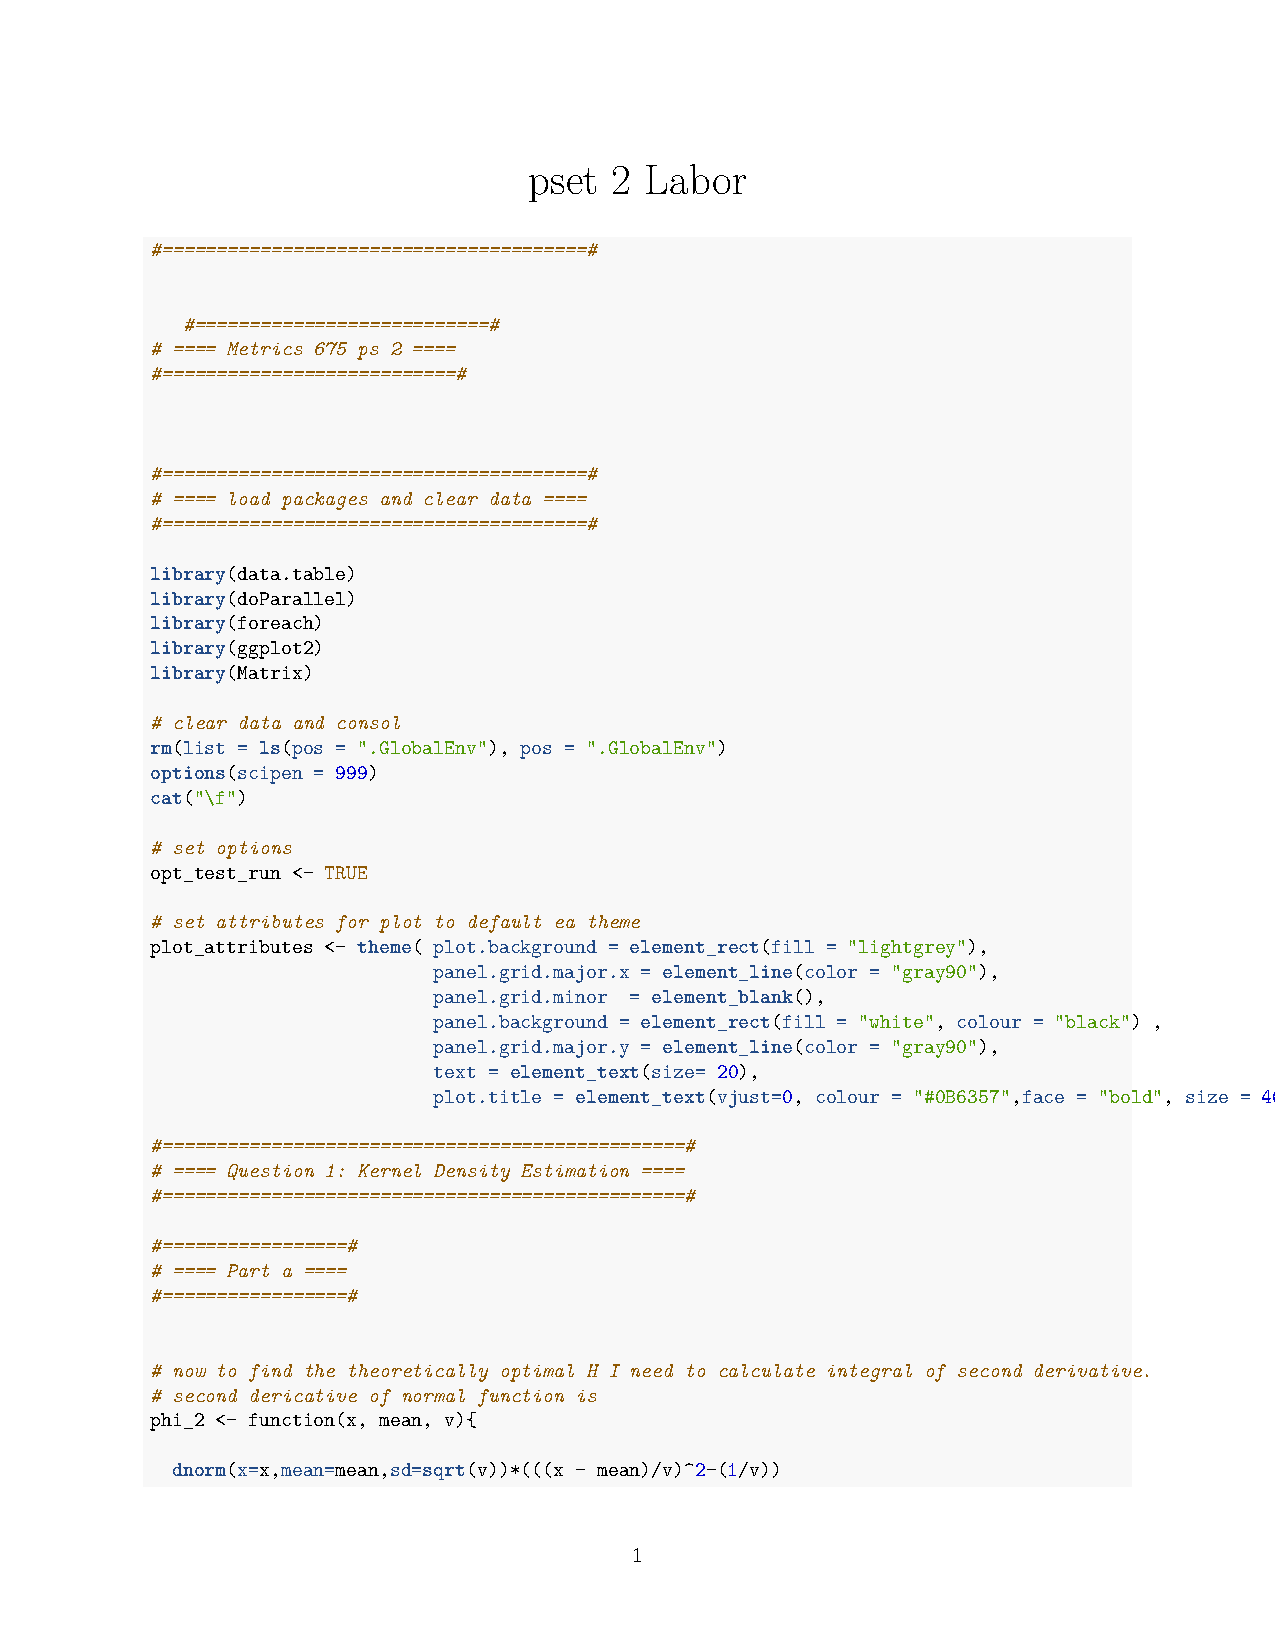
\includepdf[page=-]{ps_2_r_code_pdf.pdf}

\subsection{STATA Code}


%------------------------------------------------
% end doc
%------------------------------------------------
\end{document}


